\chapter{Web design}
% Introduction
\writer{Paulo Fontes}
The web interface layout was built with the help of different interaction design sessions, used in Interaction Design 1 and Web Technologies 1 courses. With the help of this courses, the web page layout was built in HTML and the user experience was improved from the feedback of the interaction design sessions. The web sites graphical layout analysis and implementation is not explained or documented in this report, it can be seen in the appendix EWEB1 and EIDE1.
\p
The interface is now converted to a dynamic web interface with the use of client and server side scripting languages as JavaScript and PHP. The web interface application is running and the user experience improved, the requirements from the client were accomplished.
%
\section{Server setup}
A web server is set up in time box 4. This will contain the web interface application and can be access at the AU-Herning network at the address: http://10.1.18.223/ .

\section{Database}
The database have to be consistent and flexible enough for the scalability of the system. A database model was developed in cooperation with the other teams in the class, so a common and consistent database can be design and implemented. 
\p
In time box 7 the final model of the database was design and implemented in MySQL using the tool phpMyAdmin. The databsse can be access inside AU-Herning network at the address: http://10.1.18.223/phpMyAdmin. For evaluation reasons a user with read only privileges was created with username: eval and passwords: ede10eval.
\p
The final database model can be seen bellow with all the necessary relationships between tables.
\begin{figure}[H]
	\begin{centering}
		%\missingfigure{Updated timebox figure}
		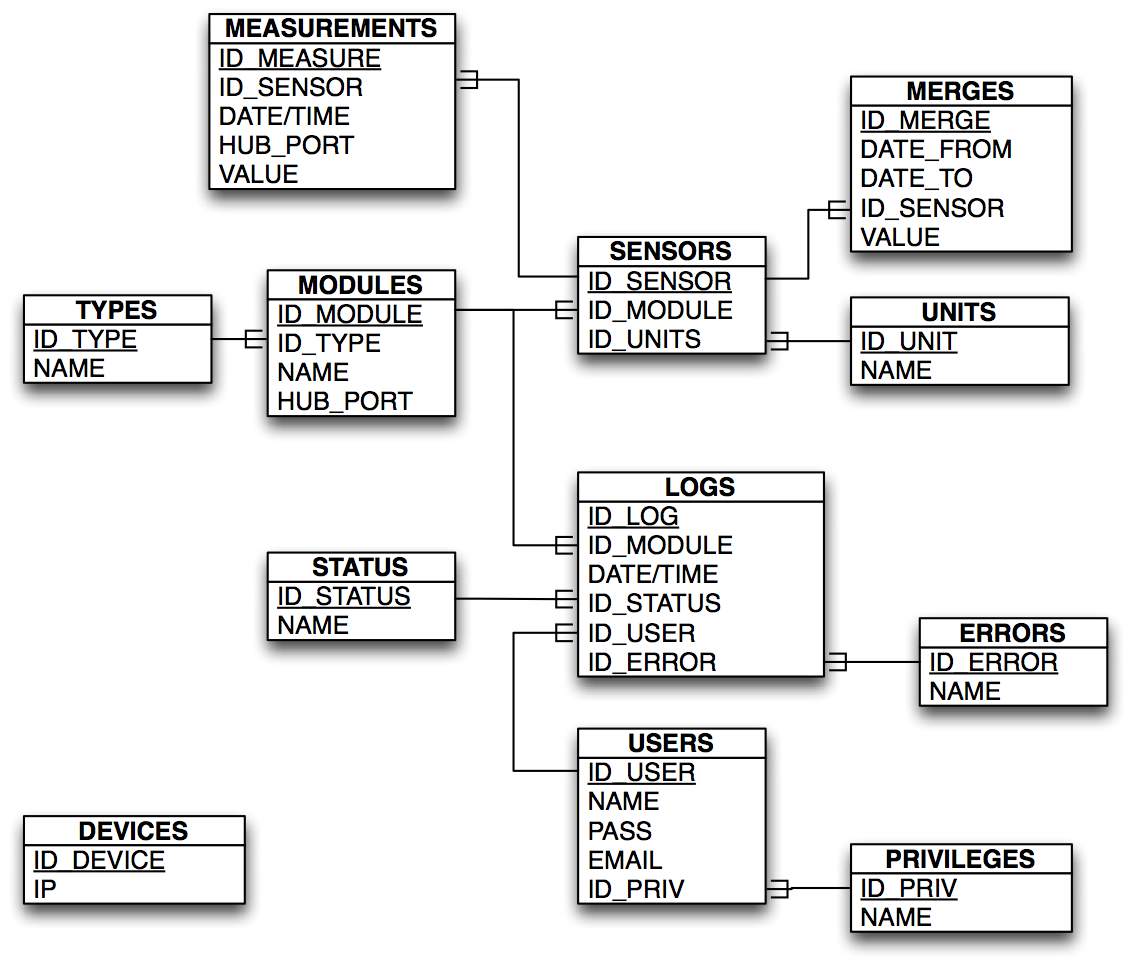
\includegraphics[width=1.0\textwidth]{images/db_datamodel.png}
		\caption{Database structure and relationships}
	\end{centering}
\end{figure}
%
\section{File structure}
Among with the database, the file structure is designed in cooperation with the other teams. Deeper analysis was made, as result the file structure was updated with new scripts added to keep the dynamics of the web interface. Error handling and user experience are important functionalities when developing a web interface application they were implemented in the end interface.
\p
The file structure used can be seen using an extra web application developed for evaluation. It can be access in the AU-Herning network at the address: http://10.1.18.223/SeeIt/.
\begin{figure}[H]
	\begin{centering}
		%\missingfigure{Updated timebox figure}
		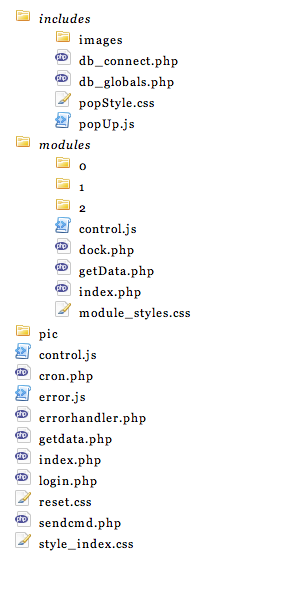
\includegraphics[width=0.3\textwidth]{images/file_structure.png}
		\caption{File structure}
	\end{centering}
\end{figure}
%
\subsection{Core Scripts}
From the developed scripts, four of them are of great importance. This scripts allow the communication between the web interface and the energy hub, retrieve data from the database to be show to the user and handle errors regarding communication to the energy hub and connection to the database.

\paragraph{Get Data}
This scripts expects a unique parameter, the id of the module or sensor which data should be retrieved. It establishes the connection to the database and using several SQL statements it returns an XML response to the client side script, that will update the data in the layout of the interface. The implementation of this script is describe in time box 7.
\p
Parameters: unique\_id have to be send as and URL encoding POST request, it will return a XML file.
\paragraph{Save Data}
The energy hub gets measurements constantly from the modules through the Power line communication, this is an UART communication type and have to be converted for something meaningful to the web world. An application running in background on the energy hub ensures that the data retrieved from the modules is translate to a HTTP request to the savedata.php script. The script will make the necessary capture from the parameters send and add a new entry to the database. The implementation of this scripts is explained in time box 6, with a new functionality added that will allow the energy hub to update the status of a port.
\p
This script is called by the GET encoding request:
\p
savedata.php \\
?sensor\_id=\textless ID Sensor\textgreater \\
\&value=\textless Sensor Measurement\textgreater \\
\&hub\_port=\textless Hub Port \textgreater
\p
or 
\p
savedata.php\\
?op=status \\
\&id\_module=\textless MODULE ID\textgreater \\
\&id\_status=\textless STATUS TO CHANDE TO\textgreater \\
\&hub\_port=\textless HUB\_PORT \textgreater
\p
Script parameters:
\begin{itemize}
	\item sensor\_id - Id of the sensor to where save data.
	\item value - the vlue to be saved
	\item hub\_port - the connected port of the module
	\item op - status, change status of a module. <unique\_id><new status>, this are add to the log table.
\end{itemize}
\paragraph{Send Commands}
The ability to send commands to the energy hub is a fundamental for the control of the system by the administrator. By the user interface the administrator have to be able to control the modules (for example change wind turbine rotation, break the wind turbine blades, etc.) and start or stop the modules connected to the energy hub.
\p
The script will wait for a answer from the energy hub if the command was routed successful or not, if not the administrator is alerted.
\p
The implementation of this script can be seen in time box 6. The script was updated since a result from the energy hub is now retrieved so the web interface application can alert the user in case error during the commands.
\p
The script is called by a encoding request method GET to:
\p
sendcmd.php \\
?id\_module=\textless Module id\textgreater \\
\&cmd=\textless Command to be send\textgreater
\p
Script parameters:
\begin{itemize}
	\item id\_module - Id of the module to send the command.
	\item cmd - command to be sent.
\end{itemize}
\paragraph{Error Handling}
Error handling is of great importance in this web interface, it alerts the user for a malfunction of the connection to the database and/or communication to the energy hub. This script is called recursively by a client side script, returning a XML response. When a error occurs in the system the error handle will change the value of a session variable, the user will be alerted to this error and the functionalities in the energy hub will be limited until the error is solved. The analysis and implementation of this script can be seen in time box 7.
